% !TeX root = ../Project.tex
\section{JEPA+SIGReg Architecture}
\label{app:jepa-sigreg-architecture}

\begin{figure}[htbp]
\centering
\includegraphics[width=\linewidth]{figures/methods/JEPA_SIGReg.pdf}
\caption{JEPA+SIGReg architecture. A shared encoder processes the masked context and complete target views, while a cross-attention predictor predicts the selected target-residue latents. Training combines the prediction loss with SIGReg.}
\label{fig:methods-jepa-sigreg-architecture}
\end{figure}

\clearpage
% !TeX root = ../Project.tex
\section{Downstream Results for Proteins up to 256 Residues}
\label{app:l256}
Table~\ref{tab:results-stb-l256} reports StructTokenBench results for proteins with at most 256 residues.
\begingroup
\ifdefined\stbworkshopbox\else\newsavebox{\stbworkshopbox}\fi
\providecommand{\stbworkshopfit}{\ifdim\wd\stbworkshopbox>\linewidth\resizebox{\linewidth}{!}{\usebox{\stbworkshopbox}}\else\usebox{\stbworkshopbox}\fi}
\begin{table}[H]
\centering
\resultstableformat
\setlength{\tabcolsep}{3pt}
\renewcommand{\arraystretch}{0.92}
\captionsetup{font=small,skip=5pt}
\fontsize{8.5}{10}\selectfont
\caption{StructTokenBench evaluation restricted to proteins with at most 256 residues.}
\label{tab:results-stb-l256}
\sbox{\stbworkshopbox}{%
\begin{tabular}{@{}lllrrrrrrrr@{}}
\toprule
\multirow{2}{*}{Task type} & \multirow{2}{*}{Task} & \multirow{2}{*}{Split} & \multicolumn{2}{c}{Autoencoders} & \multicolumn{3}{c}{JEPA} & \multicolumn{3}{c}{JEPA+SIGReg} \\[1.8pt]
 & & & $C_\alpha$ & Full AE & 50\% & 70\% & Mut. & 50\% & 70\% & Mut. \\
\midrule
\multicolumn{11}{c}{\textbf{Functional-site prediction: AUROC $\times100$}} \\
\midrule
\multirow{5}{*}{Binding site} & \multirow{2}{*}{BindInt} & Fold & 41.69 & 40.66 & 40.54 & 42.03 & \textbf{42.14} & 38.91 & 40.65 & 39.69 \\
 &  & SF & 86.84 & 85.80 & 87.39 & 86.07 & 86.82 & \textbf{89.52} & 83.70 & 88.85 \\
 & \multirow{2}{*}{BindBio} & Fold & 62.96 & \textbf{65.32} & 55.60 & 58.54 & 57.47 & 57.12 & 57.47 & 57.16 \\
 &  & SF & 63.23 & \textbf{65.63} & 58.22 & 60.02 & 59.49 & 59.60 & 59.79 & 59.73 \\
 & BindShake & Test & 59.19 & \textbf{65.11} & 53.76 & 64.42 & 63.89 & 59.73 & 59.96 & 60.83 \\
\multirow{4}{*}{Catalytic site} & \multirow{2}{*}{CatInt} & Fold & 58.97 & \textbf{61.19} & 58.92 & 58.09 & 59.94 & 59.38 & 58.19 & 57.39 \\
 &  & SF & 76.50 & \textbf{76.82} & 73.79 & 75.37 & 75.36 & 74.33 & 75.91 & 76.47 \\
 & \multirow{2}{*}{CatBio} & Fold & 64.01 & \textbf{71.89} & 54.46 & 62.41 & 60.40 & 53.05 & 51.54 & 51.53 \\
 &  & SF & 78.31 & \textbf{84.44} & 65.48 & 71.96 & 69.87 & 62.06 & 61.68 & 63.21 \\
\multirow{2}{*}{Conserved site} & \multirow{2}{*}{Con} & Fold & 57.20 & \textbf{59.98} & 59.51 & 58.51 & 59.34 & 58.85 & 59.43 & 59.22 \\
 &  & SF & 71.97 & 73.48 & 70.73 & 71.22 & 72.43 & \textbf{74.30} & 74.10 & 74.11 \\
\multirow{2}{*}{Repeat motif} & \multirow{2}{*}{Rep} & Fold & 65.38 & 64.43 & 66.08 & 65.91 & 65.37 & \textbf{67.73} & 66.97 & 67.08 \\
 &  & SF & 80.79 & 79.82 & \textbf{82.00} & 79.24 & 81.25 & 77.65 & 76.02 & 77.46 \\
\multirow{2}{*}{Epitope region} & \multirow{2}{*}{Ept} & Fold & 56.28 & 55.21 & \textbf{59.29} & 54.79 & 56.57 & 58.34 & 56.67 & 55.90 \\
 &  & SF & 64.15 & 62.59 & \textbf{65.09} & 60.61 & 61.86 & 61.02 & 60.76 & 57.63 \\
\midrule
\multicolumn{11}{c}{\textbf{Remote homology: macro-F1 $\times100$}} \\
\midrule
\multirow{3}{*}{Remote homology} & \multirow{3}{*}{Homo} & Fold & 7.89 & 6.29 & 7.10 & \textbf{10.21} & 8.77 & 7.43 & 7.98 & 8.54 \\
 &  & Family & \textbf{35.26} & 26.86 & 17.67 & 21.29 & 17.00 & 21.52 & 20.01 & 26.60 \\
 &  & SF & 8.41 & 10.47 & 4.97 & \textbf{11.59} & 8.51 & 7.73 & 6.67 & 6.14 \\
\midrule
\multicolumn{11}{c}{\textbf{Structural flexibility: Spearman's $\rho\times100$}} \\
\midrule
\multirow{6}{*}{Flexibility} & \multirow{2}{*}{FlexRMSF} & Fold & 14.98 & \textbf{45.34} & 26.50 & 30.46 & 30.76 & 12.12 & 10.48 & 10.31 \\
 &  & SF & 13.96 & \textbf{44.34} & 31.68 & 28.47 & 33.10 & 10.26 & 10.24 & 8.45 \\
 & \multirow{2}{*}{FlexBFactor} & Fold & 11.21 & \textbf{26.00} & 1.80 & 19.62 & 16.25 & 1.91 & 3.32 & 2.80 \\
 &  & SF & 11.26 & \textbf{26.94} & 12.97 & 22.10 & 23.40 & 4.01 & 3.56 & 4.92 \\
 & \multirow{2}{*}{FlexNEQ} & Fold & 15.98 & 24.95 & 10.52 & \textbf{33.38} & 16.92 & 7.98 & 7.75 & 7.80 \\
 &  & SF & 13.51 & 22.11 & 11.43 & \textbf{29.19} & 10.87 & 6.61 & 6.82 & 6.63 \\
\bottomrule
\end{tabular}%
}
\stbworkshopfit
\end{table}

\clearpage
\endgroup

% !TeX root = ../Project.tex
\section{Supporting Result Diagnostics}
\label{sec:results-supporting}

Figures~\ref{fig:appendix-reconstruction-examples} and~\ref{fig:appendix-reconstruction-failures} show additional whole-protein reconstructions and representative local failure modes.

\begin{figure}[H]
\centering
\captionsetup{font=small,skip=3pt}
\begin{minipage}[t]{0.48\linewidth}
  \centering
  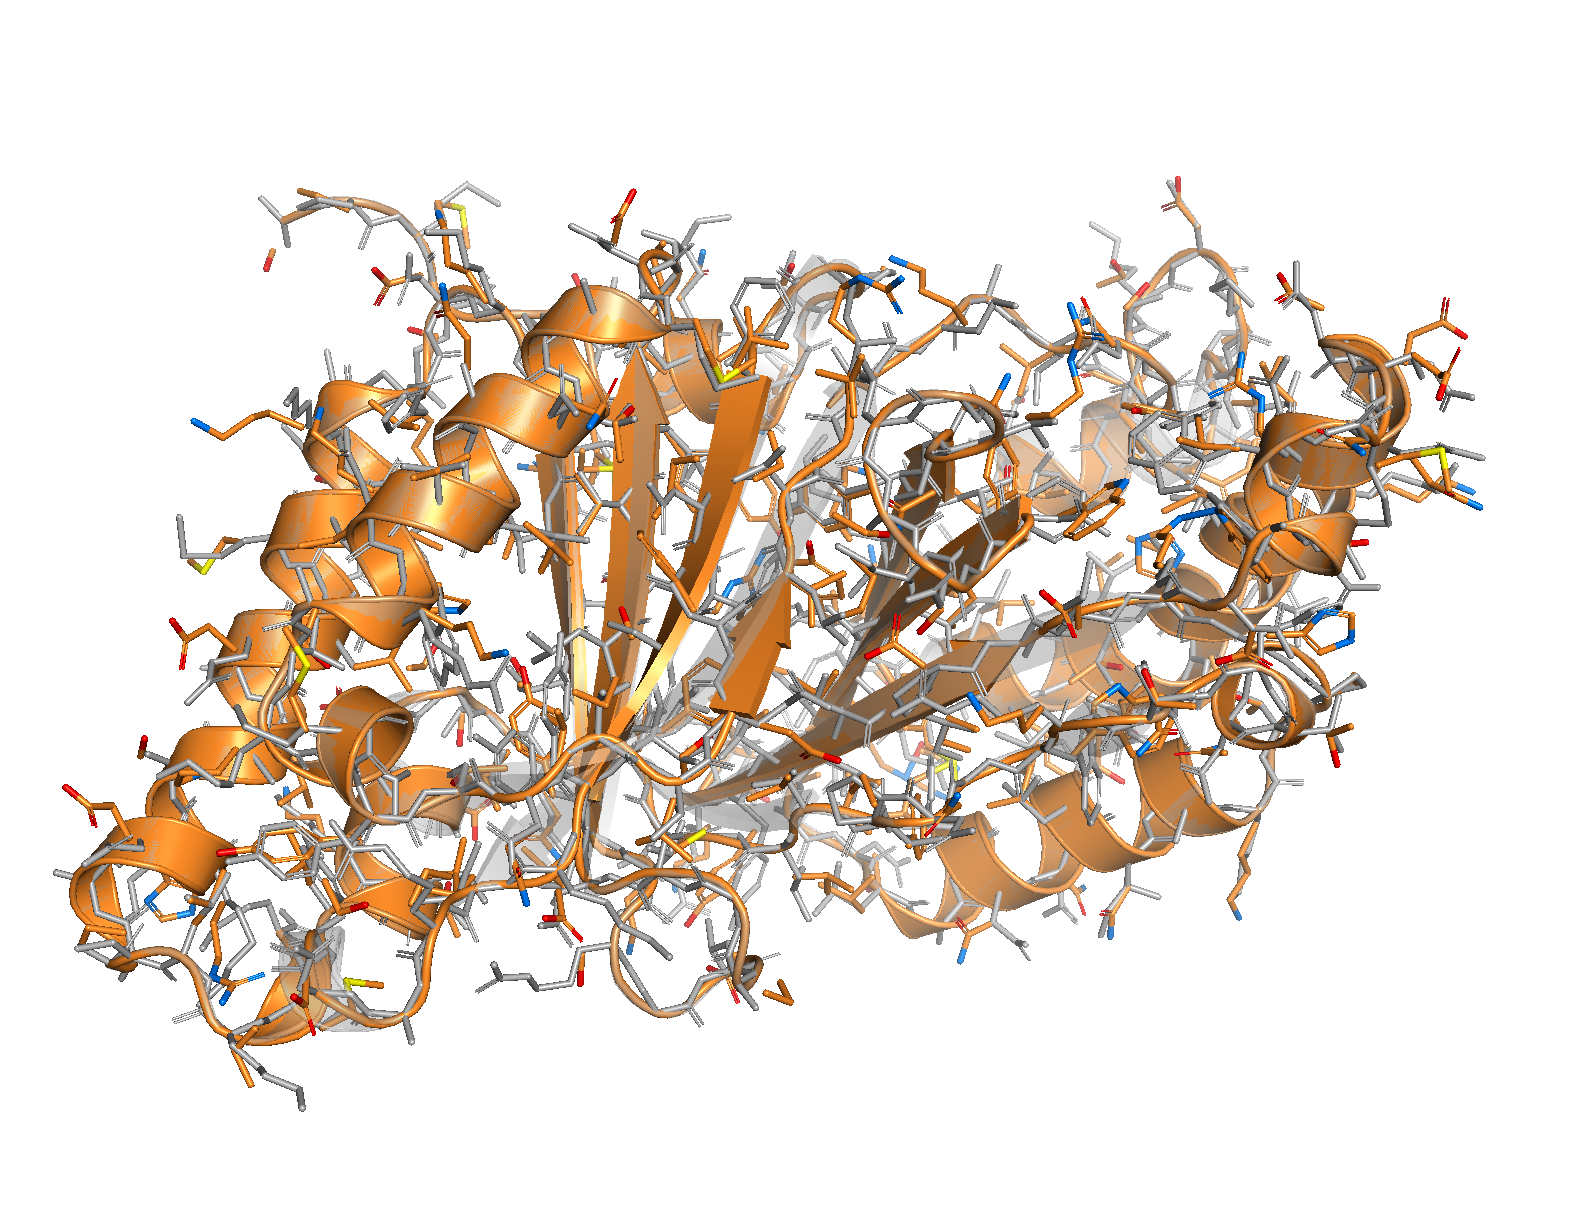
\includegraphics[height=0.14\textheight]{figures/protein_figures/5a13_G.png}\\[-2pt]
  \small (a) 5A13 chain G
\end{minipage}\hfill
\begin{minipage}[t]{0.48\linewidth}
  \centering
  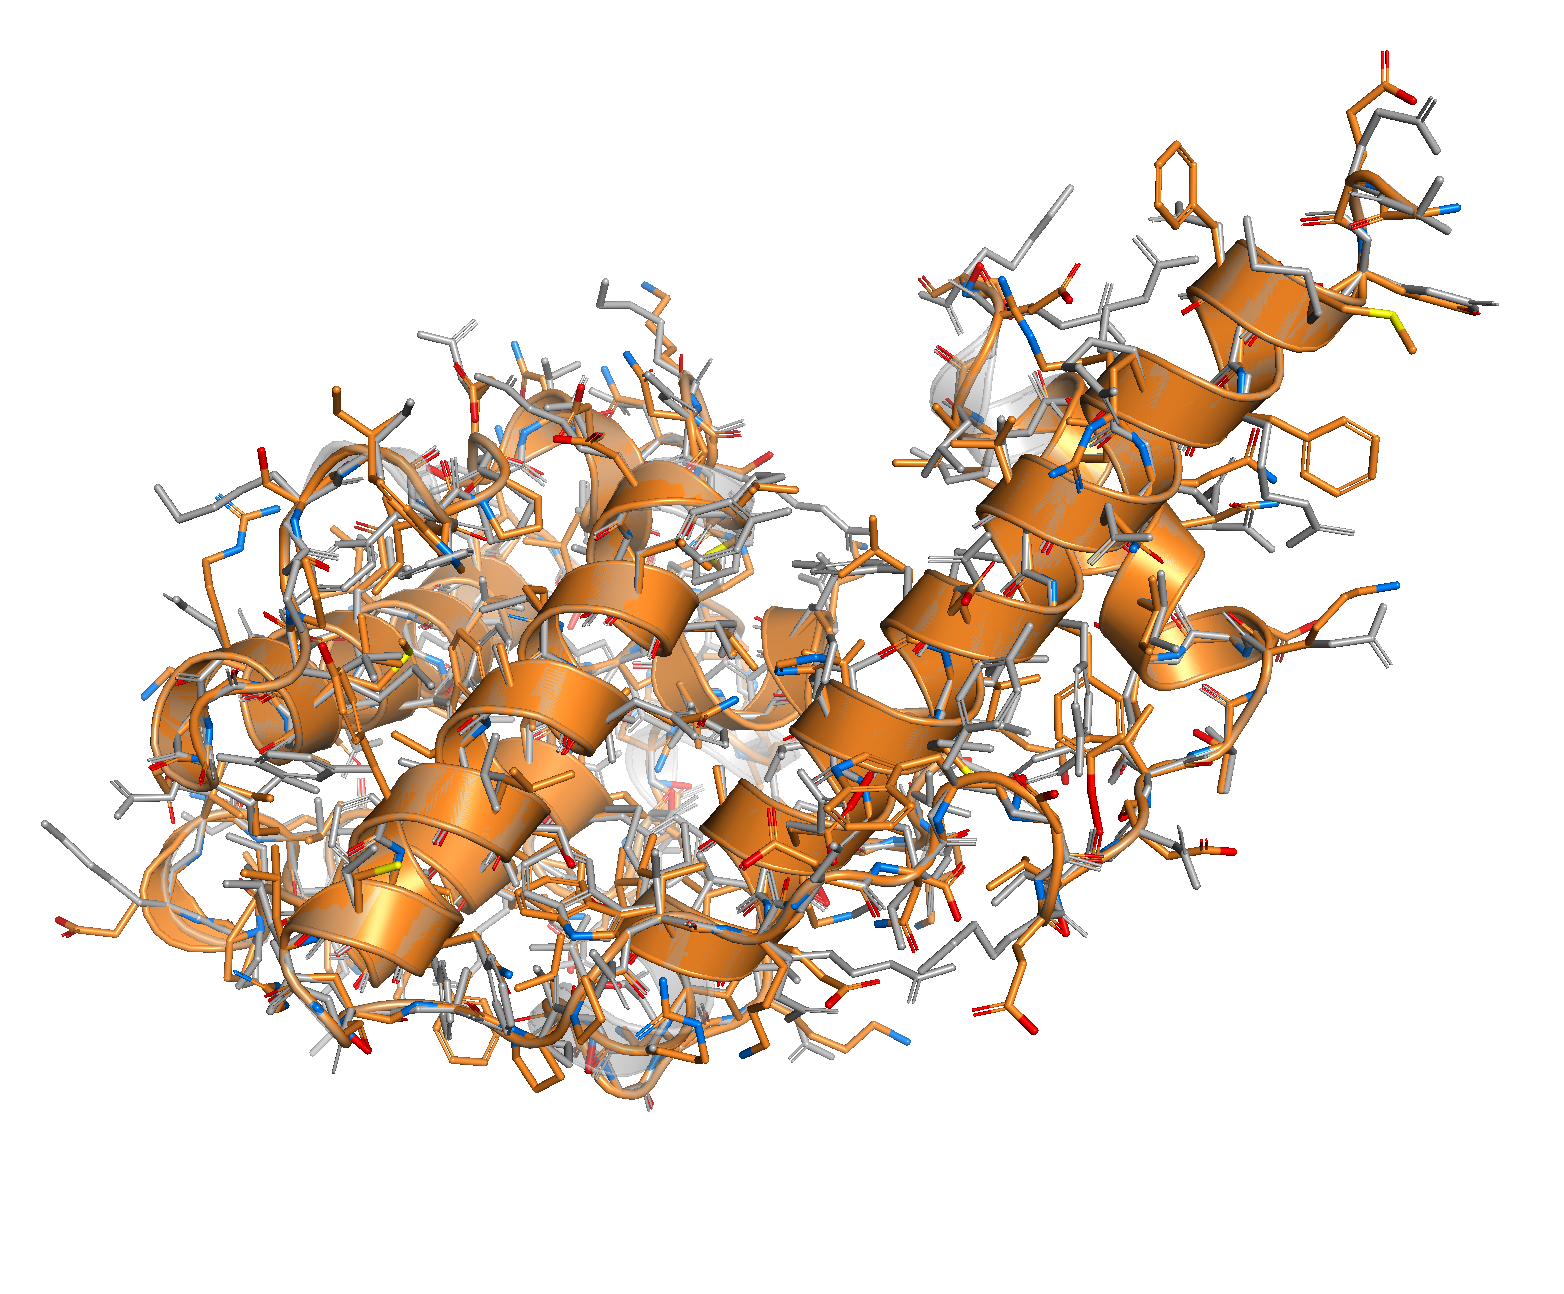
\includegraphics[height=0.14\textheight]{figures/protein_figures/5l0o_A.png}\\[-2pt]
  \small (b) 5L0O chain A
\end{minipage}

\vspace{2pt}
\begin{minipage}[t]{0.48\linewidth}
  \centering
  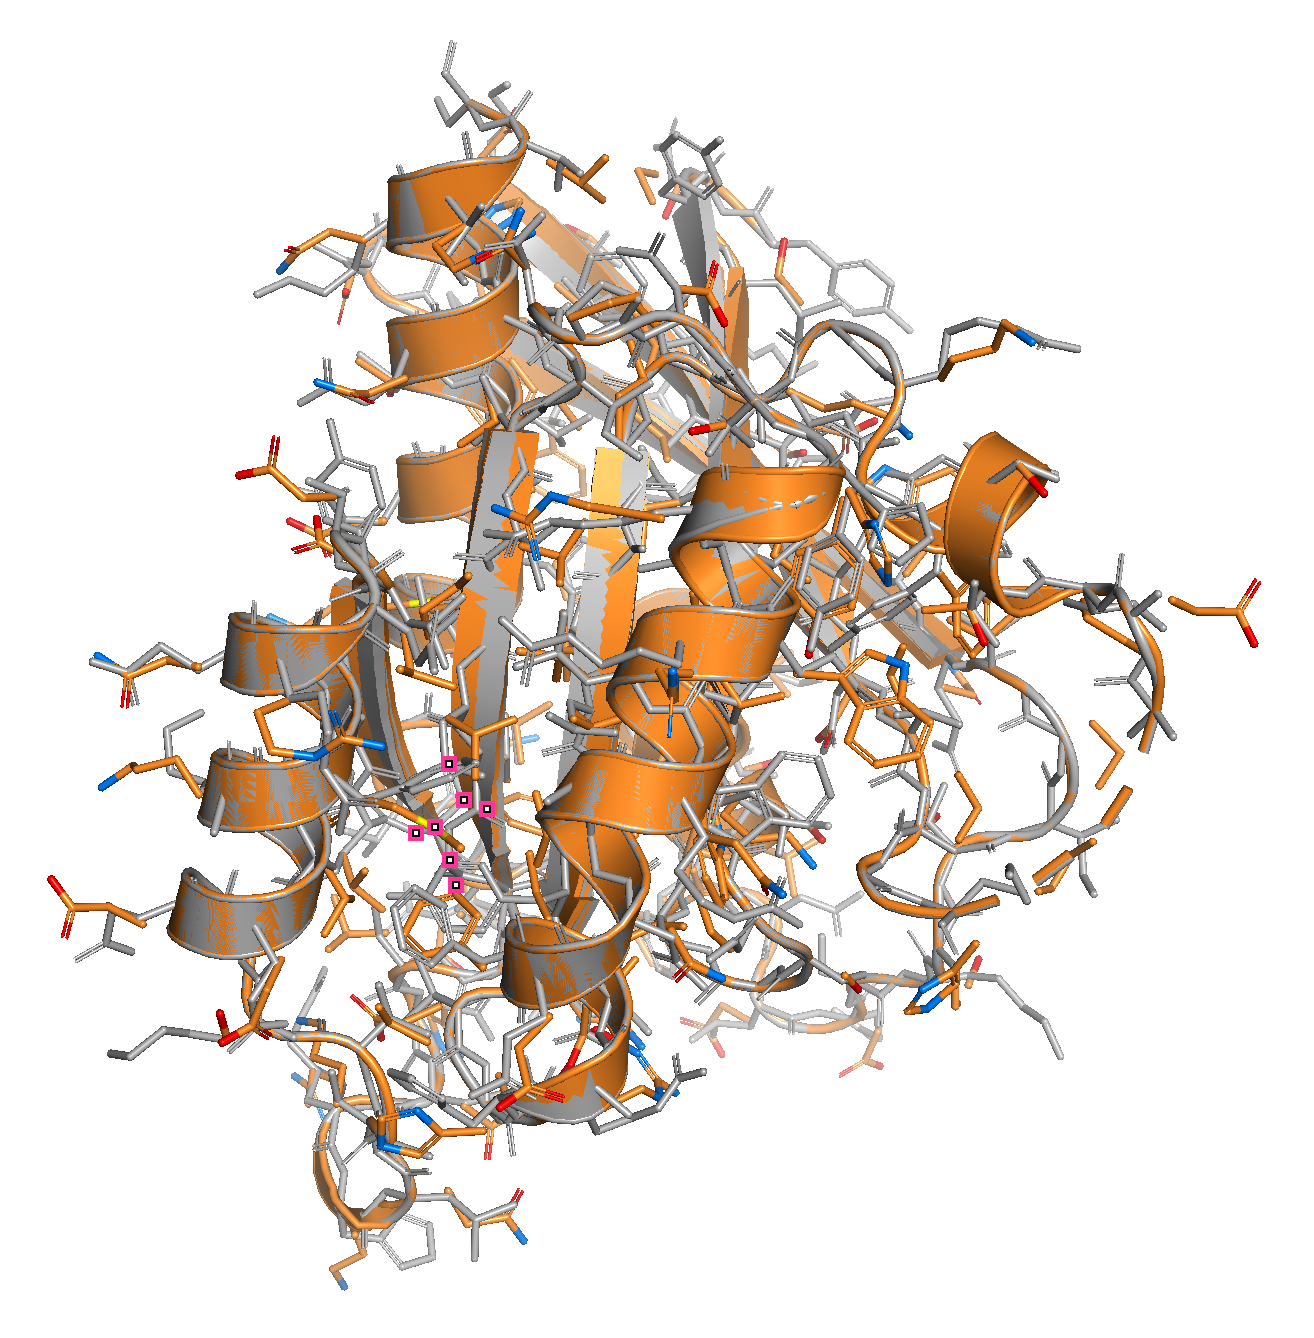
\includegraphics[height=0.14\textheight]{figures/protein_figures/5xr7_A.png}\\[-2pt]
  \small (c) 5XR7 chain A
\end{minipage}\hfill
\begin{minipage}[t]{0.48\linewidth}
  \centering
  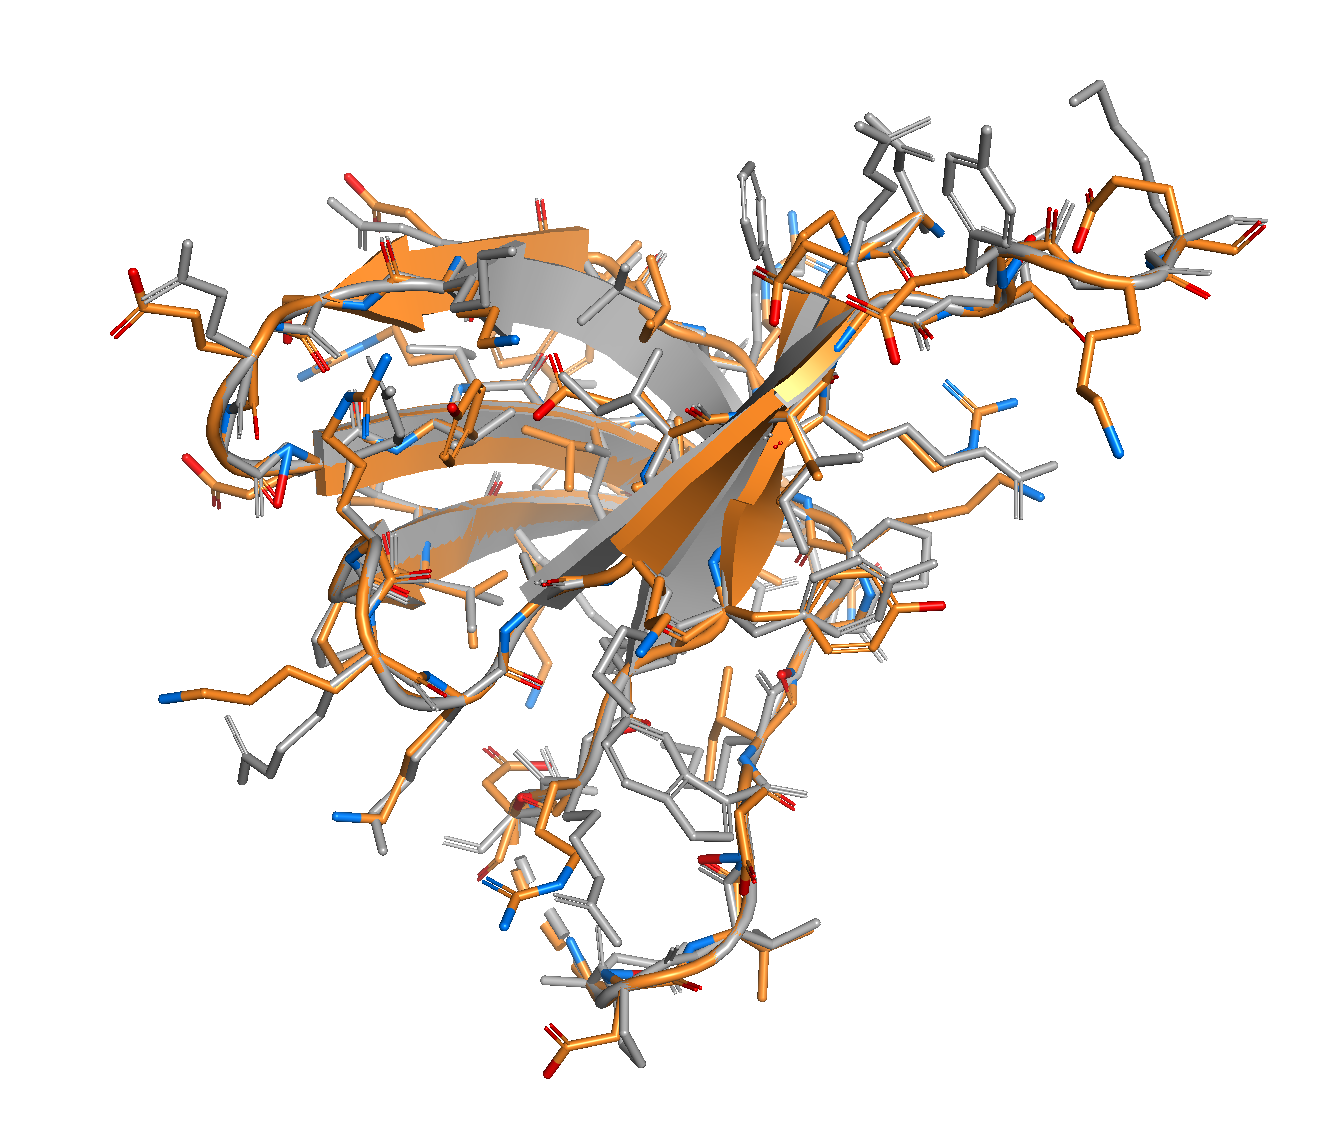
\includegraphics[height=0.14\textheight]{figures/protein_figures/8cbv_A.png}\\[-2pt]
  \small (d) 8CBV chain A
\end{minipage}
\caption{Whole-protein overlays of native structures in grey and postprocessed JEPA reconstructions in orange.}
\label{fig:appendix-reconstruction-examples}
\end{figure}

\begin{figure}[H]
\centering
\captionsetup{font=small,skip=3pt}
\begin{minipage}[t]{0.48\linewidth}
  \centering
  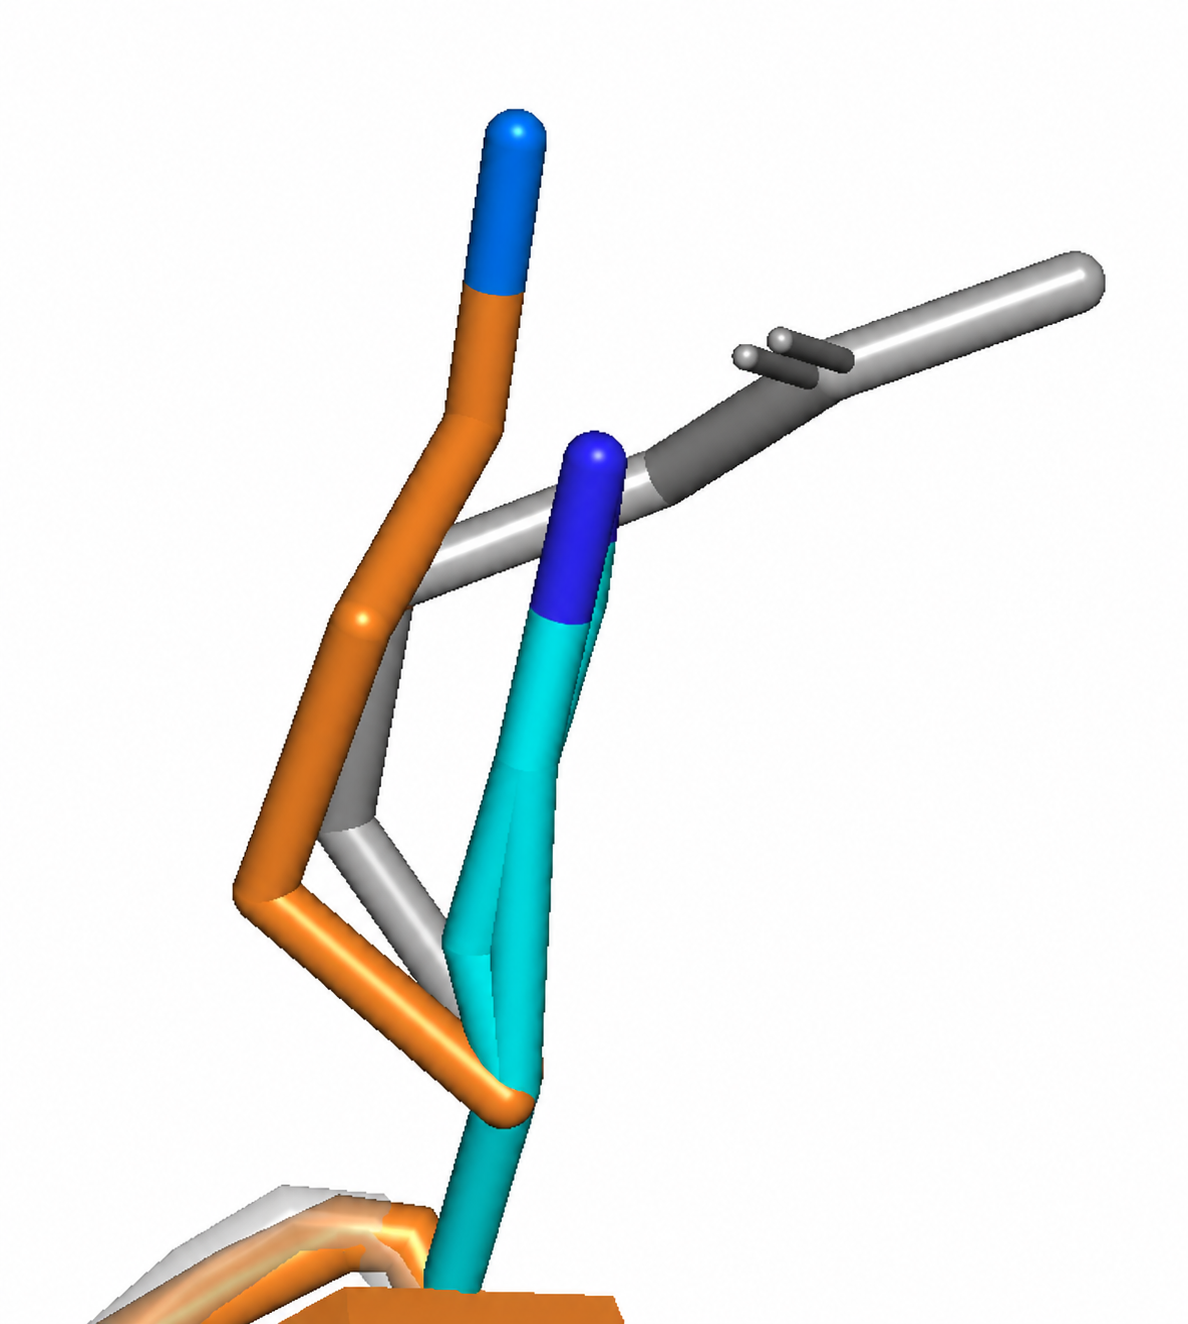
\includegraphics[height=0.14\textheight]{figures/protein_figures/fm1-clean.png}\\[-2pt]
  \small (a) Distorted bond geometry
\end{minipage}\hfill
\begin{minipage}[t]{0.48\linewidth}
  \centering
  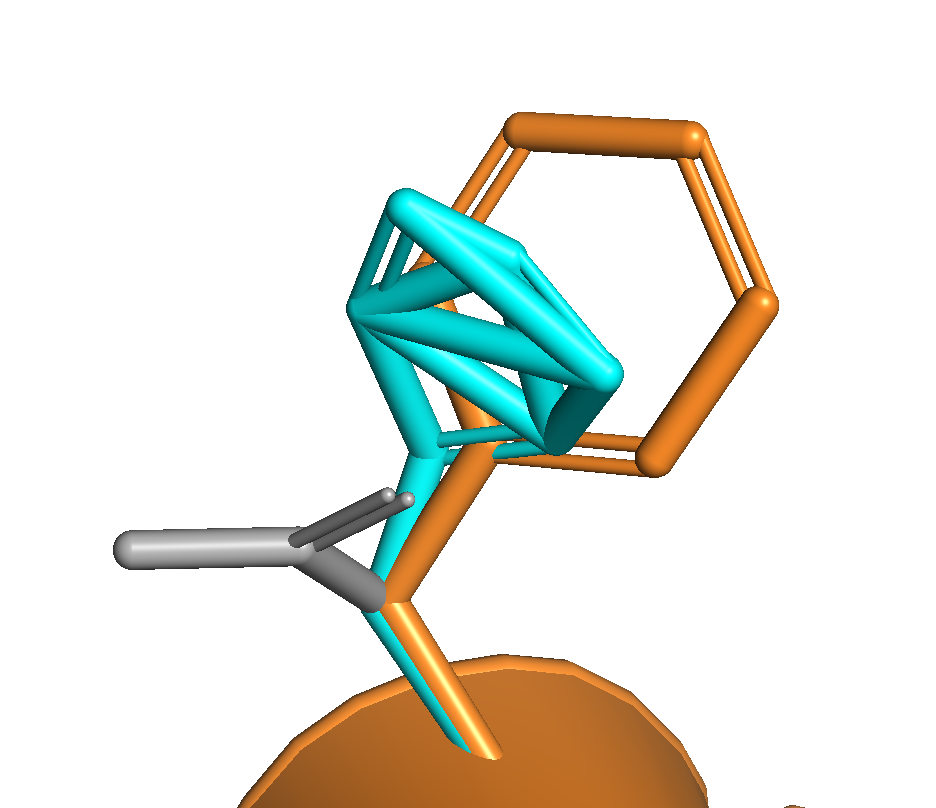
\includegraphics[height=0.14\textheight]{figures/protein_figures/fm2.png}\\[-2pt]
  \small (b) Overlapping side-chain atoms
\end{minipage}

\vspace{2pt}
\begin{minipage}[t]{0.48\linewidth}
  \centering
  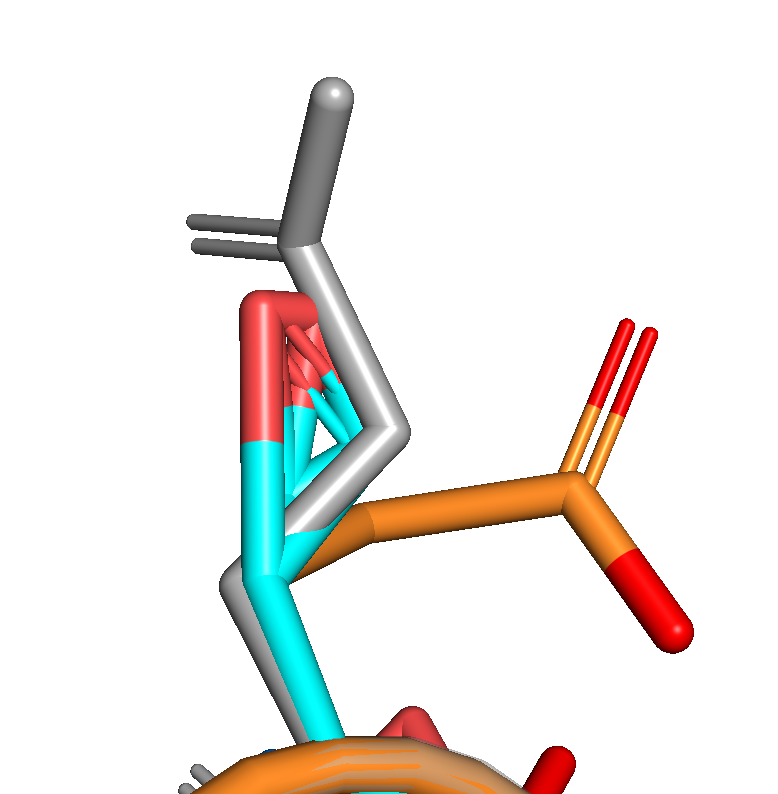
\includegraphics[height=0.14\textheight]{figures/protein_figures/fm3.png}\\[-2pt]
  \small (c) Misplaced side-chain atoms
\end{minipage}\hfill
\begin{minipage}[t]{0.48\linewidth}
  \centering
  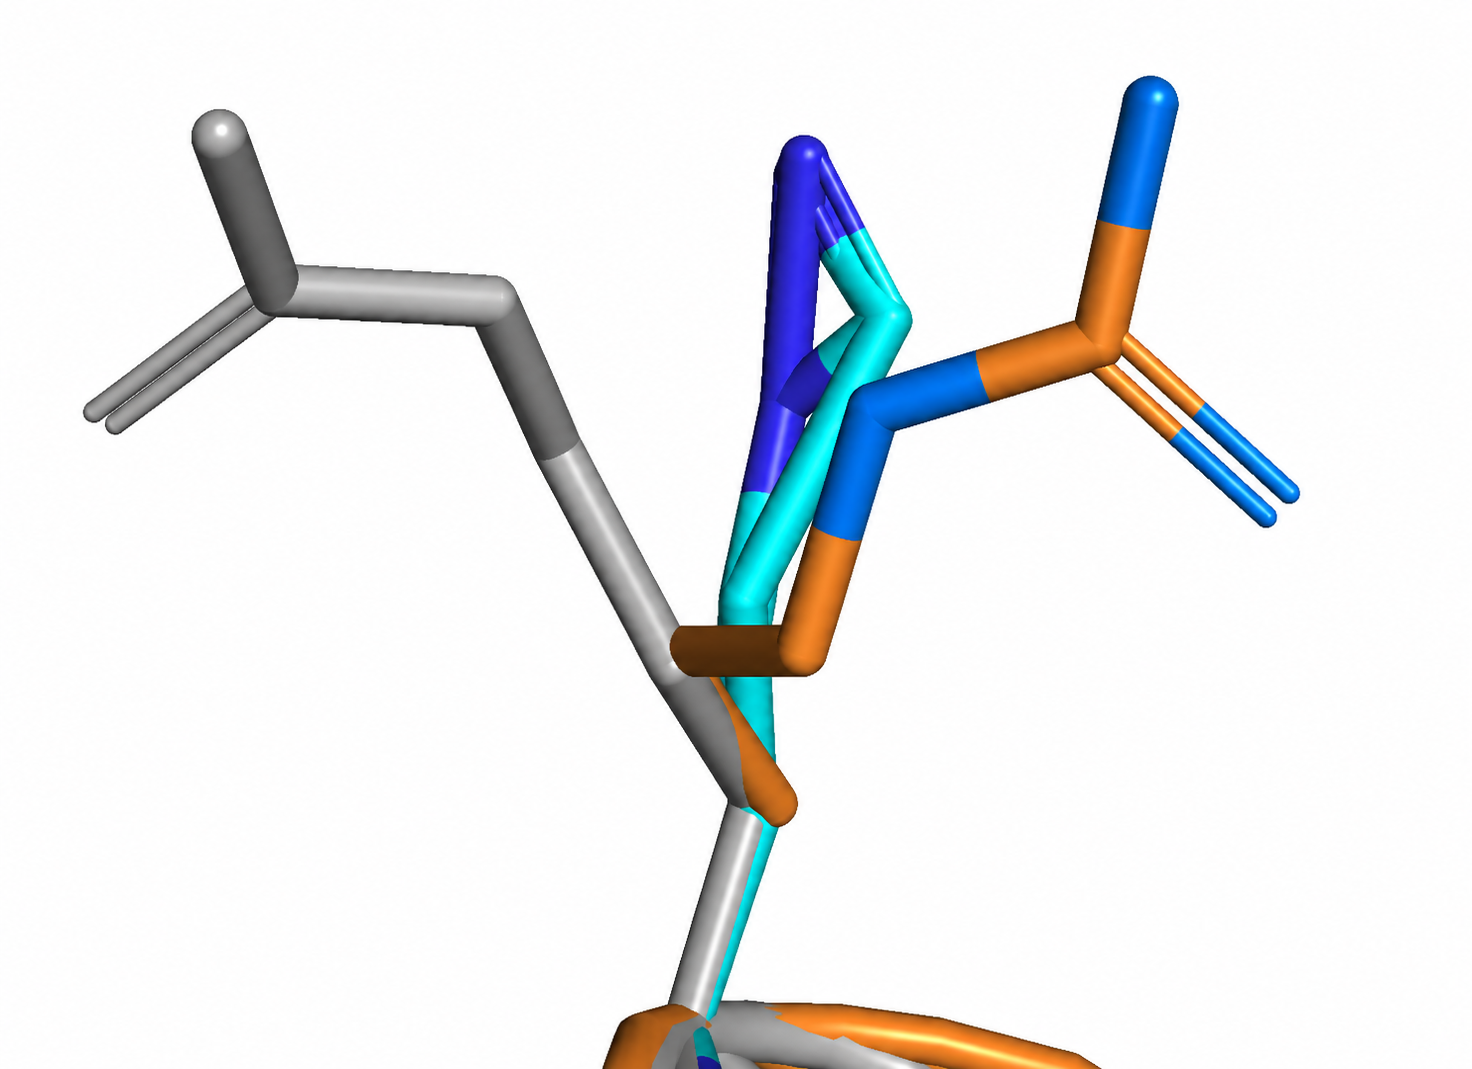
\includegraphics[height=0.14\textheight]{figures/protein_figures/fm4-clean.png}\\[-2pt]
  \small (d) Distorted local connection
\end{minipage}
\caption{Examples of local geometric failure modes. Native structures are grey, postprocessed JEPA predictions are orange, and direct decoder outputs are cyan.}
\label{fig:appendix-reconstruction-failures}
\end{figure}


\clearpage
\section{Latent-Space Model and Design Comparisons}
\label{app:latent-figures}

\begin{figure}[H]
\centering
\captionsetup{font=small,skip=3pt}
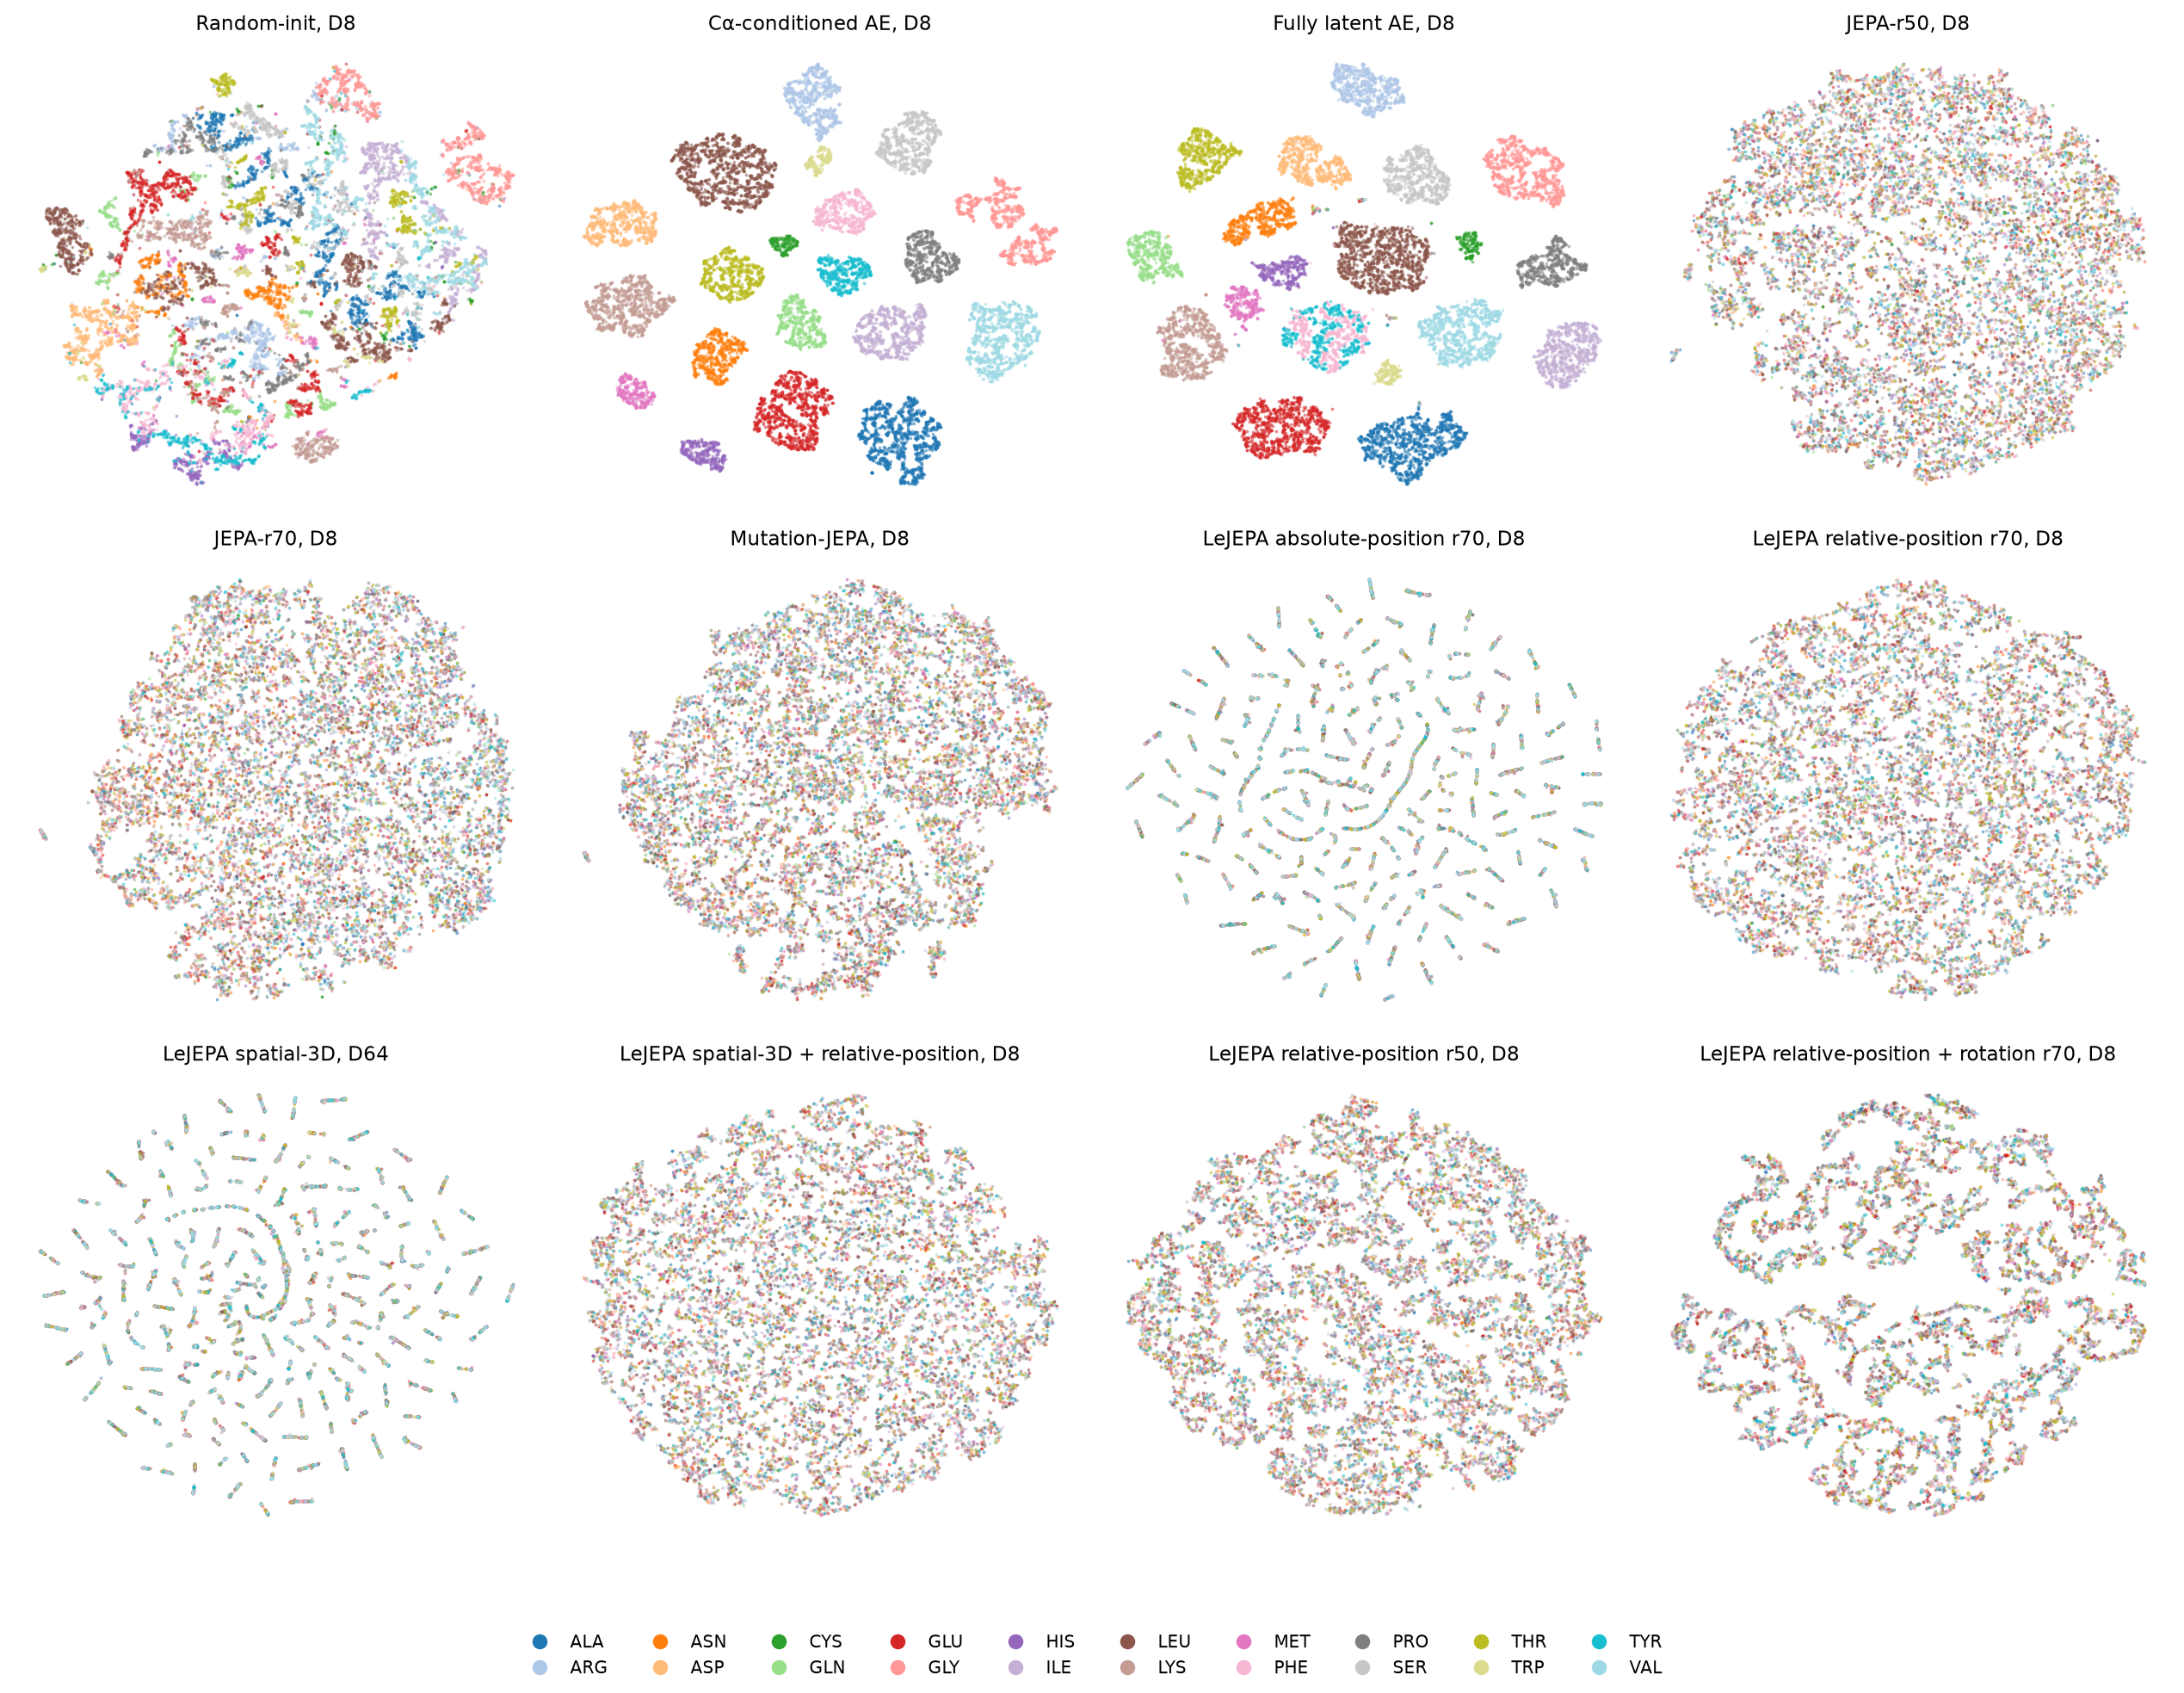
\includegraphics[width=\linewidth]{figures/results/tsne_full12_exact.png}
\caption{Per-residue t-SNE for the full 100k model roster, coloured by amino-acid identity. The same evaluation residues and visualisation settings are used across models. This figure provides qualitative latent-space context for the main L600 results.}
\label{fig:full-latent-grid}
\end{figure}

\begin{figure}[H]
\centering
\captionsetup{font=small,skip=3pt}
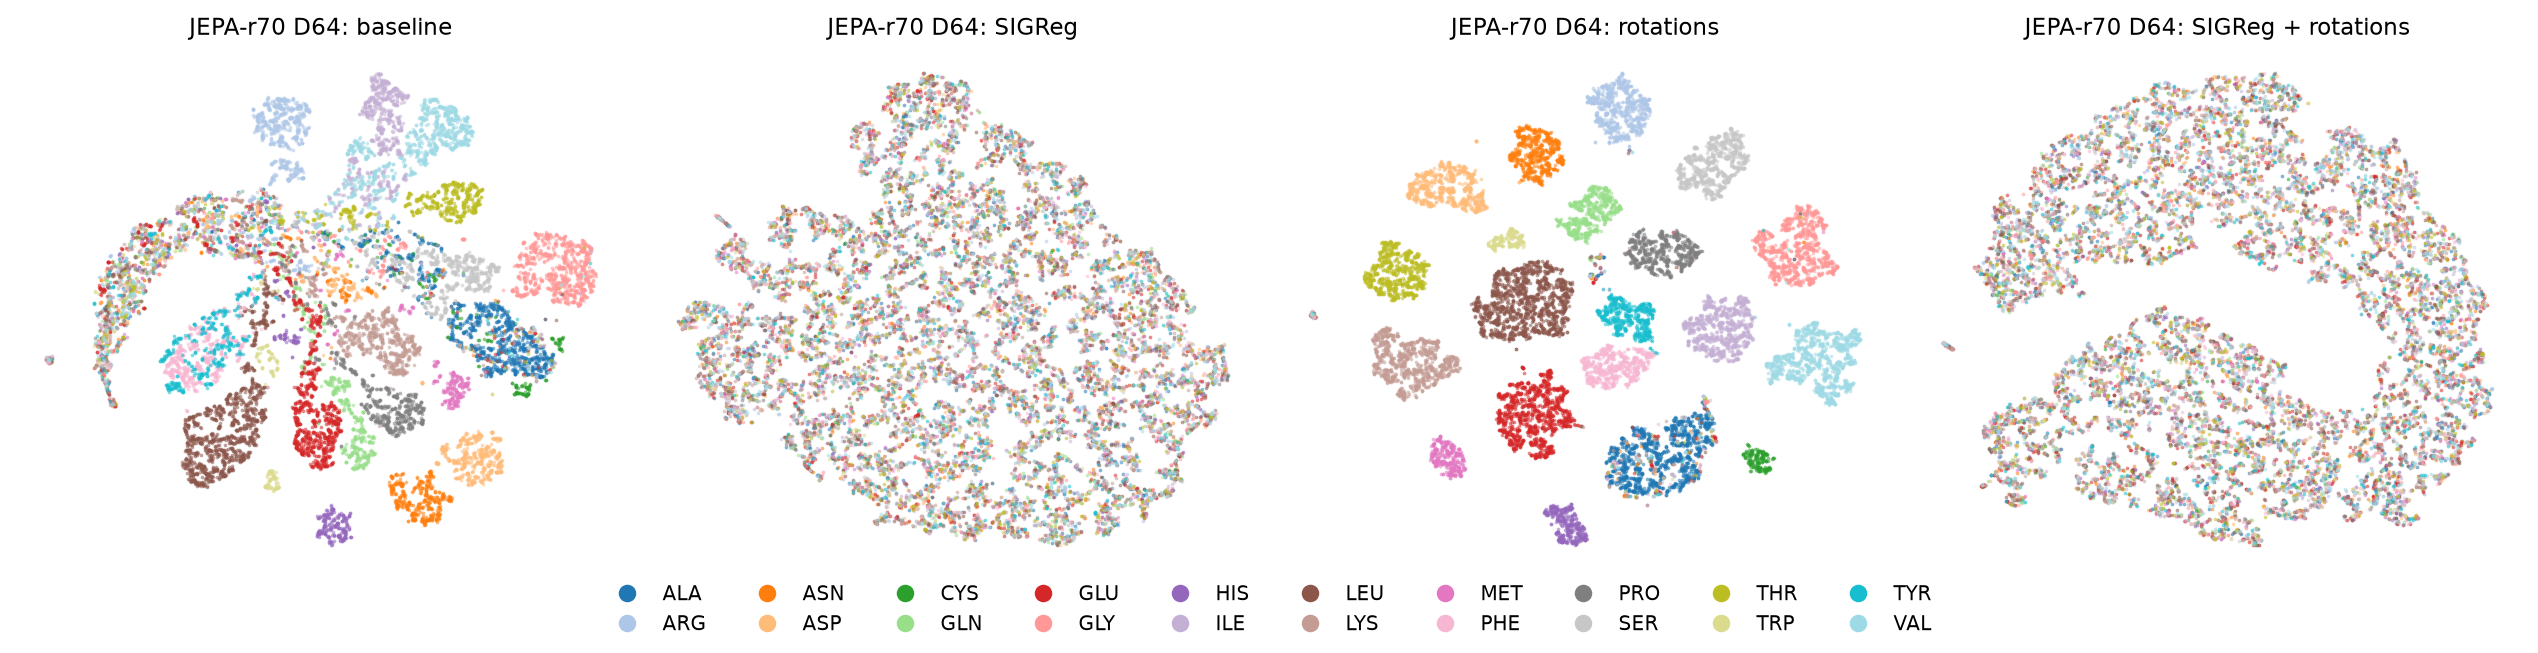
\includegraphics[width=\linewidth]{figures/results/tsne_decisions_exact.png}
\caption{Matched 10k 64D EMA-JEPA design grid: baseline, SIGReg, independent rotations, and SIGReg plus rotations. Points are coloured by amino-acid identity.}
\label{fig:decision-grid}
\end{figure}

We first show the full 100k latent-space roster used throughout the thesis. Figure~\ref{fig:full-latent-grid} compares the same evaluation-residue sample across all models. The reconstruction baselines form amino-acid-separated clusters, standard EMA-JEPA variants are more mixed, the absolute-position JEPA+SIGReg model forms repeated strands, and relative-position variants remove that structure. Random initialisation is included as an architectural control.

We then isolate two design choices in a matched 64D EMA-JEPA screen. Figure~\ref{fig:decision-grid} compares a baseline run, SIGReg, independent $\mathrm{SO}(3)$ view rotations, and SIGReg plus rotations. Rotation produces clear amino-acid clusters in this short-run comparison, whereas adding SIGReg without rotation produces a mixed representation. These visualisations motivate, but do not replace, quantitative invariance and transfer tests.

\clearpage
\section{Supporting Layerwise Evaluation}
\label{app:layerwise-supporting}
\label{app:jepa-r70-layerwise}
\begingroup
\setlength{\intextsep}{4pt}
The matched JEPA random-70 evaluation is complete at all three hidden blocks for BindInt, BindBio, BindShake, CatInt and CatBio.
Across these nine task/split scores, block 6 exceeds the final 8D latent in both model families. It is the strongest of the four readouts on 7/9 canonical LeJEPA scores and 5/9 JEPA scores (Tables~\ref{tab:results-layer-stb} and~\ref{tab:results-layer-stb-jepa-r70}).
This recurrence indicates that the middle-layer advantage is not unique to the canonical LeJEPA objective, although the JEPA results currently cover only this five-task subset.

\begin{table}[H]
\centering
\setlength{\tabcolsep}{4pt}
\renewcommand{\arraystretch}{0.86}
\captionsetup{font=small,skip=3pt}
\fontsize{9}{10.5}\selectfont
\caption{Completed layerwise STB for JEPA with 70\% random masking, using raw/online weights at 100k and full-context evaluation. Hidden-block outputs are 768D and the final latent mean is 8D. Scores are multiplied by 100. Bold marks the strongest readout for each task/split.}
\label{tab:results-layer-stb-jepa-r70}
\begin{tabular}{@{}llrrrr@{}}
\toprule
\multirow{2}{*}{Task} & \multirow{2}{*}{Split}
& \multicolumn{4}{c}{JEPA, random 70\%} \\[1.8pt]
& & Block 1 & Block 6 & Block 12 & Final 8D \\
\midrule
\multirow{2}{*}{BindInt}
& Fold & 47.86 & \textbf{48.86} & 48.24 & 47.11 \\
& SF   & 88.24 & \textbf{91.95} & 91.59 & 80.06 \\
\multirow{2}{*}{BindBio}
& Fold & 72.61 & \textbf{73.22} & 72.84 & 65.56 \\
& SF   & 72.93 & \textbf{73.85} & 73.76 & 65.31 \\
BindShake
& Test & 78.23 & 78.13 & \textbf{78.38} & 71.85 \\
\multirow{2}{*}{CatInt}
& Fold & 65.69 & \textbf{65.72} & 65.05 & 56.84 \\
& SF   & 88.00 & 91.79 & \textbf{92.00} & 76.71 \\
\multirow{2}{*}{CatBio}
& Fold & \textbf{80.72} & 80.13 & 78.23 & 71.50 \\
& SF   & 89.81 & 89.62 & \textbf{90.39} & 75.36 \\
\bottomrule
\end{tabular}
\end{table}

\begin{figure}[H]
\centering
\captionsetup{font=small,skip=3pt}
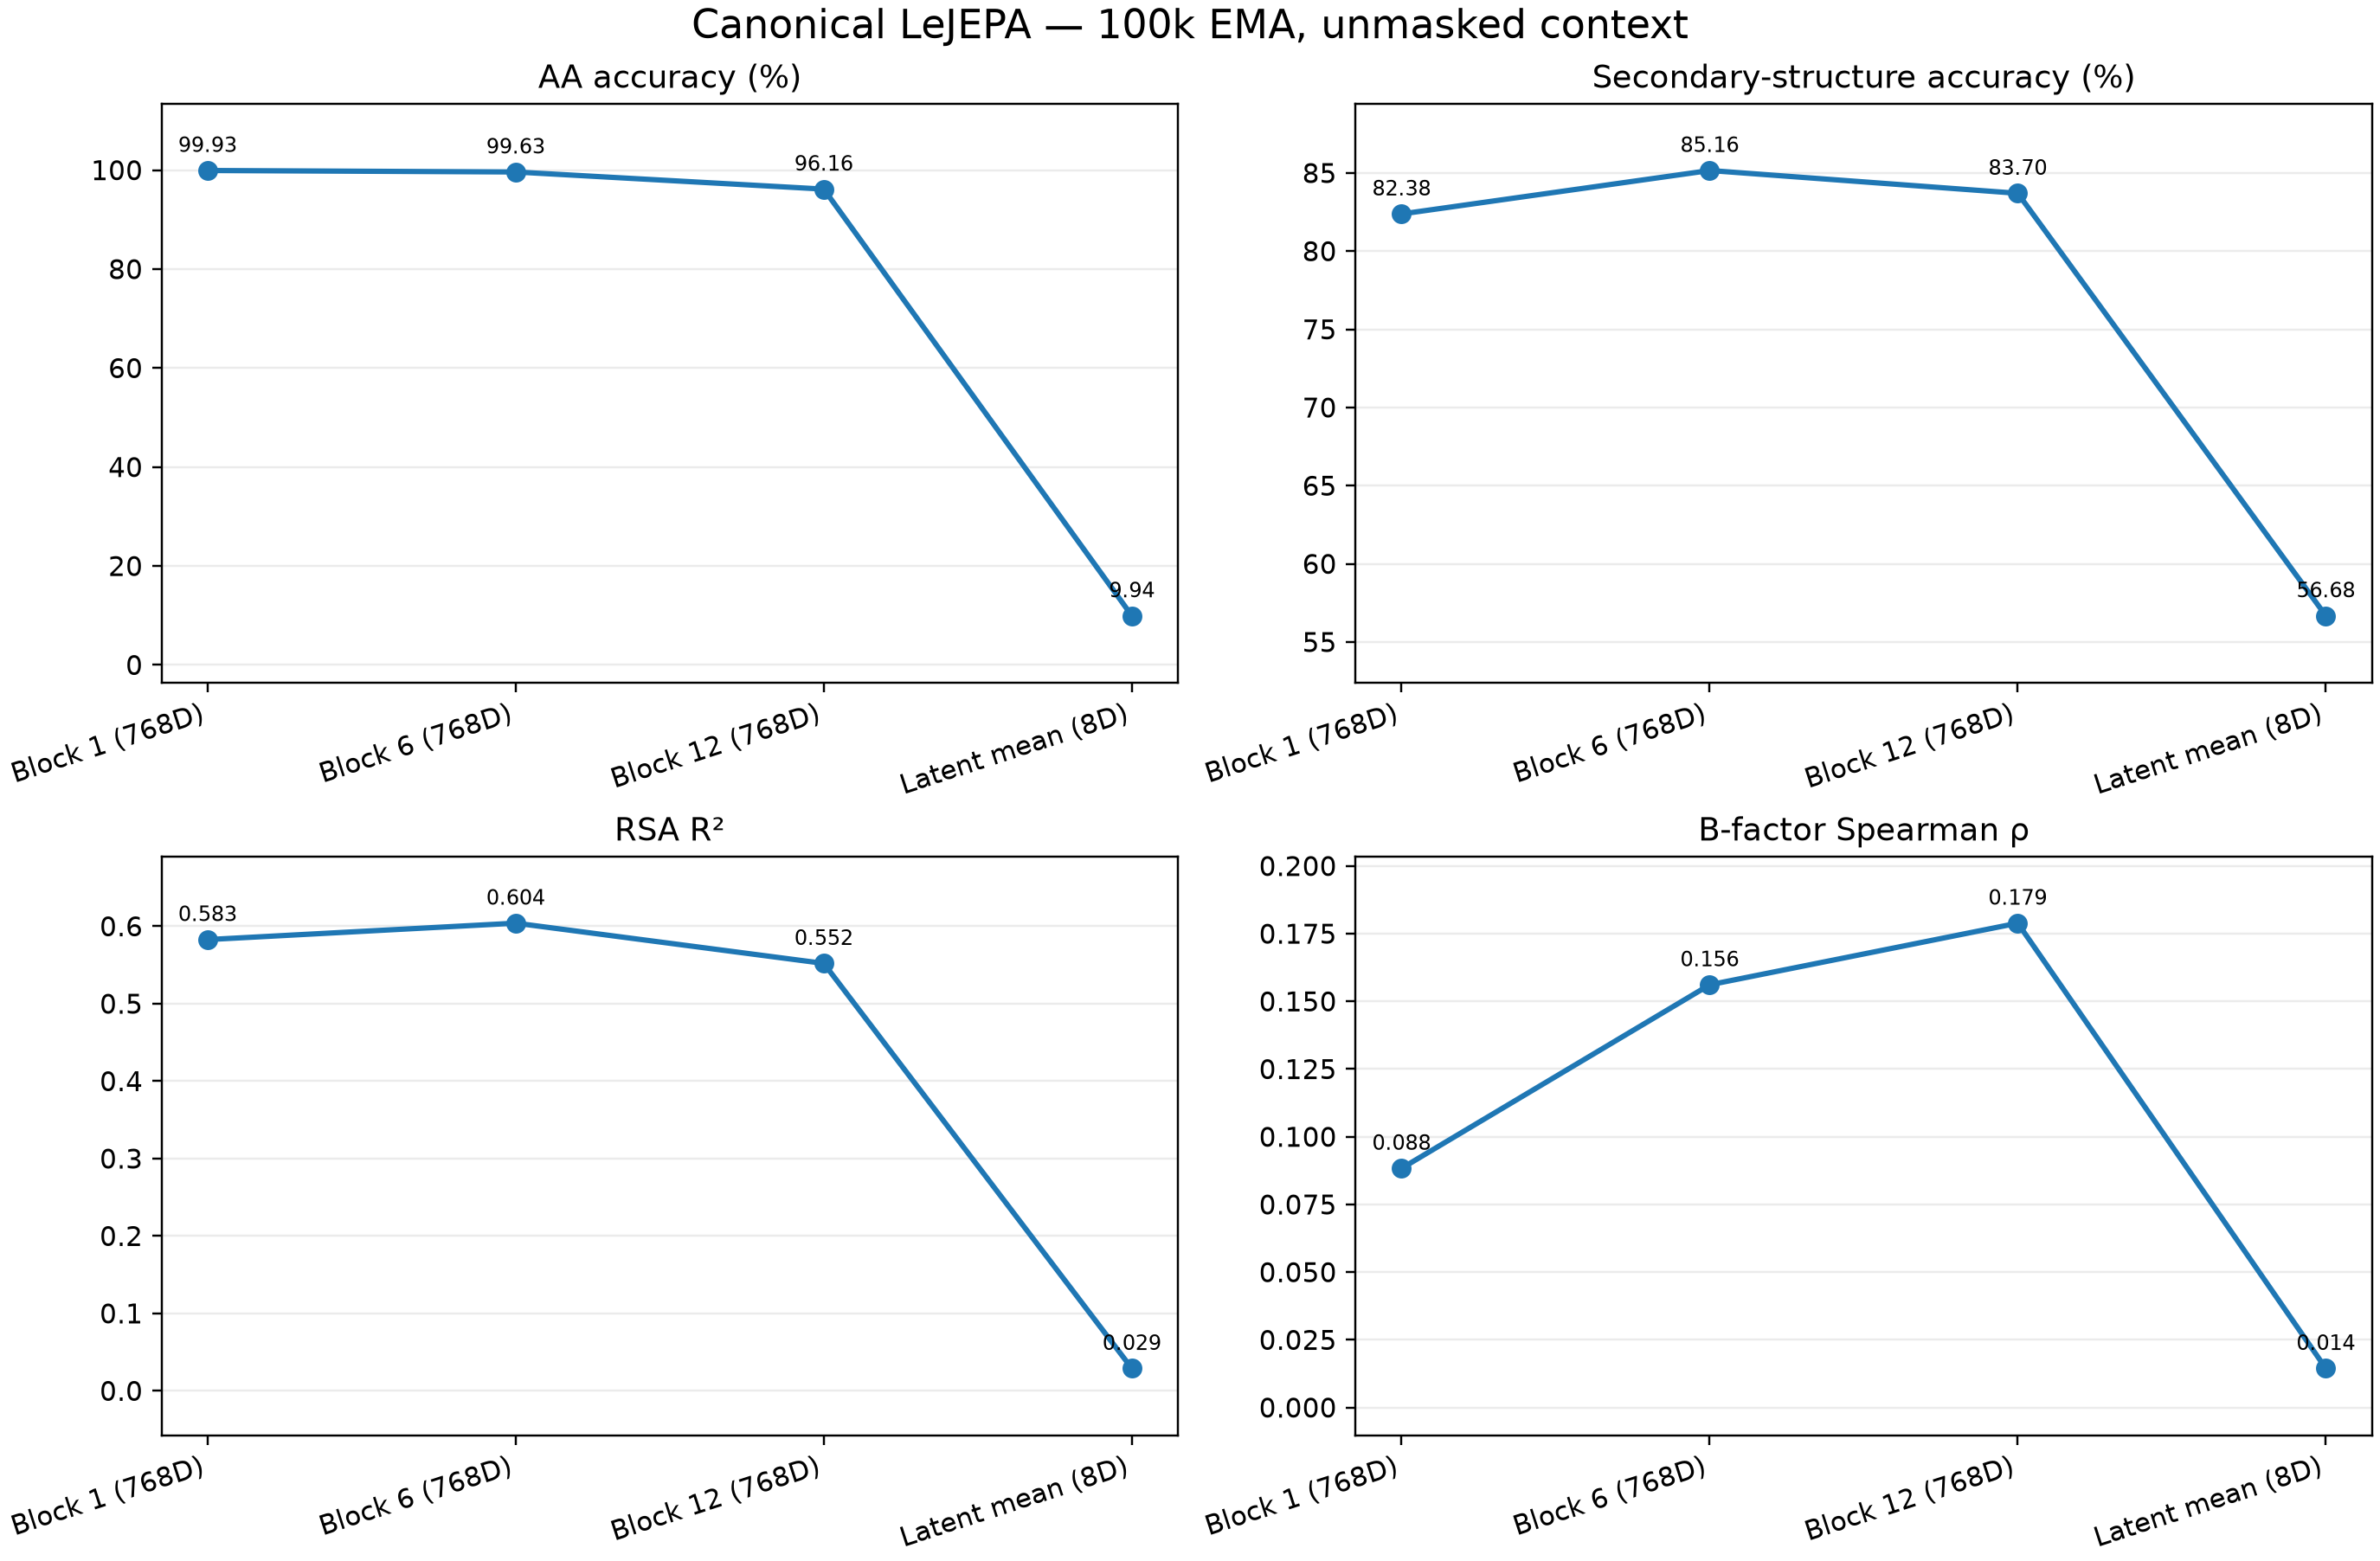
\includegraphics[width=0.80\linewidth]{figures/results/canonical_lejepa_full_context_layerwise_probes.png}
\caption{Full-context linear probes from one uncropped LeJEPA 100k EMA checkpoint. Hidden states are 768D and the final latent mean is 8D. Block-1 SS and block-12 amino-acid/SS fits reported convergence warnings. The highlighted block-6 and latent-mean SS/RSA fits did not. Lines connect different readouts, not a training trajectory.}
\label{fig:results-layer-probes}
\end{figure}
\endgroup
\clearpage

\section{Effect of Encoder Depth}
\label{app:encoder-depth}
Table~\ref{tab:results-encoder-depth} compares the final 8D latent means of separately trained six- and twelve-block uncropped LeJEPA encoders.
Both use seed 42, and the STB cohorts and downstream predictor configurations match.
Each depth was trained once, so the differences have not been checked across independent training seeds.
Training time, memory use and checkpoint sizes are not compared here.

\begin{table}[htbp]
\centering
\setlength{\tabcolsep}{6pt}
\renewcommand{\arraystretch}{0.97}
\captionsetup{font=small,skip=5pt}
\fontsize{8.8}{10}\selectfont
\caption{Full-L600 STB for uncropped LeJEPA with 12 and 6 encoder blocks, without rotations, using raw final-8D latent means at 100k. Scores are multiplied by 100. Bold marks the higher score in each row. $\Delta$ is six-block minus twelve-block. Differences and their unweighted mean across the 24 task/split scores are computed before rounding. This mixed-metric mean is descriptive, not a unified benchmark score.}
\label{tab:results-encoder-depth}
\begin{tabular}{@{}llrrr@{}}
\toprule
Task & Split & \shortstack{12-block\\Final 8D} & \shortstack{6-block\\Final 8D} & $\Delta$ \\
\midrule
\multicolumn{5}{c}{\textbf{Functional-site prediction: AUROC $\times100$}} \\
\midrule
BindInt & Fold & \textbf{50.30} & 45.81 & $-4.49$ \\
 & SF & 88.45 & \textbf{88.58} & $+0.12$ \\
BindBio & Fold & \textbf{59.32} & 59.28 & $-0.04$ \\
 & SF & \textbf{61.82} & 61.41 & $-0.40$ \\
BindShake & Test & 58.45 & \textbf{59.15} & $+0.70$ \\
CatInt & Fold & 51.71 & \textbf{57.13} & $+5.42$ \\
 & SF & \textbf{80.74} & 79.20 & $-1.54$ \\
CatBio & Fold & 53.67 & \textbf{54.06} & $+0.39$ \\
 & SF & \textbf{60.61} & 60.50 & $-0.11$ \\
Con & Fold & \textbf{60.10} & 58.07 & $-2.03$ \\
 & SF & 77.27 & \textbf{78.01} & $+0.73$ \\
Rep & Fold & 71.05 & \textbf{73.05} & $+2.00$ \\
 & SF & 83.49 & \textbf{83.64} & $+0.15$ \\
Ept & Fold & \textbf{62.00} & 54.51 & $-7.49$ \\
 & SF & \textbf{59.72} & 58.83 & $-0.89$ \\
\midrule
\multicolumn{5}{c}{\textbf{Remote homology: macro-F1 $\times100$}} \\
\midrule
Homo & Fold & 6.73 & \textbf{7.73} & $+1.00$ \\
 & Family & \textbf{19.64} & 16.70 & $-2.94$ \\
 & SF & 5.54 & \textbf{6.56} & $+1.02$ \\
\midrule
\multicolumn{5}{c}{\textbf{Structural flexibility: Spearman's $\rho\times100$}} \\
\midrule
FlexRMSF & Fold & 22.48 & \textbf{29.84} & $+7.36$ \\
 & SF & 30.96 & \textbf{41.25} & $+10.28$ \\
FlexBFactor & Fold & 5.01 & \textbf{6.54} & $+1.54$ \\
 & SF & 3.50 & \textbf{5.11} & $+1.61$ \\
FlexNEQ & Fold & 2.46 & \textbf{4.19} & $+1.73$ \\
 & SF & 3.54 & \textbf{5.21} & $+1.67$ \\
\midrule
\multicolumn{4}{l}{Mean difference (6-block $-$ 12-block)} & $+0.66$ \\
\bottomrule
\end{tabular}
\end{table}
\clearpage
